\documentclass[unknownkeysallowed, 10pt, a4 paper, handout]{beamer}

% Custom beamer theme
\usepackage{../style/beamerthemeCustom}
\newcommand{\HRule}{\rule{\linewidth}{0.5mm}}   %FOR TITLEPAGE

\usepackage{changepage}       % adjustwidth

\setlength\parskip{0.3cm}

\definecolor{darkgreen}{RGB}{0,100,0}
\newcommand{\green}[1]{\textbf{\textcolor{darkgreen}{#1}}}
\newcommand{\red}[1]{\textbf{\textcolor{red}{#1}}}

\newcommand{\focus}[1]{\textbf{\textcolor{red}{#1}}}
\newcommand{\ra}{$\longrightarrow$ }
\newcommand{\lra}{$\longleftrightarrow$ }

\newcommand{\code}[1]{\colorbox{black}{\color{green}\texttt{#1}}}

% Command to create two side-by-side minipages
\newcommand{\sidebyside}[5]{
  \begin{minipage}{#1\textwidth}
    #2
  \end{minipage} #3 \begin{minipage}{#4\textwidth}
    #5
  \end{minipage}
}

\begin{document}

\begin{frame}[label=permission]{File permissions}
  \begin{columns}[T]
    \begin{column}{.11\textwidth}
      \includegraphics[scale=0.15]{pics/Timbro.jpg}
    \end{column}
    \hfill
    \begin{column}{.89\textwidth}
      \small{
      There are three basic attributes for plain file permissions:
      \begin{itemize}
         \item read
         \item write
         \item execute
      \end{itemize}
      They mean what you would expect. There are three classes of users:
      \begin{itemize}
         \item owner
         \item group
         \item other
      \end{itemize}
      For each of the three classes you have three possible attributes
      to set. \\
      \vspace{10pt}
      For directories:
      \begin{itemize}
         \item read : you can list the content
         \item write : you can create/remove files inside
         \item execute : you can access it and its content
      \end{itemize}
    }
    \end{column}
  \end{columns}
\end{frame}


\begin{frame}
  \begin{center}
    \frametitle{Check permissions}

    \sidebyside{0.44}{
      \centering
      See permissions: \code{ls -l}
    }{\hfill}{0.52}{
      \begin{center}
        \includegraphics[width=1.00\textwidth]{pics/ls-l.png}
      \end{center}
    }

    First 3 chars: \focus{read} (\code{r}), \focus{write} (\code{w}), \focus{execute} (\code{x}) permissions \focus{for user}\\
    Second 3 chars: read/write/execute \focus{for group}\\
    Last 3 chars: read/write/execute \focus{for all users}

    Useful if the system does not leave you remove a file
  \end{center}
\end{frame}


\begin{frame}
  \begin{center}
    \frametitle{Changing permissions: \code{chmod}}

    \sidebyside{0.42}{
      Change permissions: \code{chmod}

      \code{chmod <who><+/-><what> <file>}

      \begin{itemize}
        \item \code{<who>}:\\
          \code{u} (user),\\
          \code{g} (group),\\
          \code{a} (everybody)
        \item \code{<+/->}: \code{+} to add, \code{-} to remove
        \item \code{what}: \code{r,w,x} as above
      \end{itemize}
    }{\hfill}{0.48}{
      \begin{center}
        \includegraphics[width=0.90\textwidth]{pics/chmod.png}
      \end{center}
    }
  \end{center}
\end{frame}


\begin{frame}
  \begin{center}
    \frametitle{Basic shell scripting}

    As said before, you can \focus{recycle} commands you use more than once:\\
    \focus{write once, use more than once}

    \sidebyside{0.50}{
      You can create \focus{scripts}:\\
      files containing instructions\\
      which you launch to perform tasks
    }{\hfill}{0.45}{
      \begin{center}
        \includegraphics[width=0.70\textwidth]{pics/script_1.png}
      \end{center}
    }

    \begin{itemize}
      \item The first line tells the shell which \focus{interpreter} to use\\
        (i.e. which scripting language, we use \code{bash})
      \item The rest is \focus{instructions} (this here prints 'hello')
    \end{itemize}

    \sidebyside{0.50}{
      Scripts can be made \focus{executable}\\
      (remember \code{chmod}?)\\
      and launched from the command line:\\
      \code{./<script>}
    }{\hfill}{0.45}{
      \begin{center}
        \includegraphics[width=0.80\textwidth]{pics/script_2.png}
      \end{center}
    }
  \end{center}
\end{frame}

\begin{frame}
  \begin{center}
    \frametitle{Executing scripts and programs}

    \sidebyside{0.45}{
      \centering
      \code{./<executable>}\\
      \focus{launches an executable}
    }{\hfill}{0.50}{
      \begin{center}
        \includegraphics[width=0.80\textwidth]{pics/execute.png}
      \end{center}
    }

   \sidebyside{0.48}{
      \centering
      \code{./<executable> \&}\\
      executes \focus{in the background}\\
      (the shell is free during execution)
    }{\hfill}{0.50}{
      \begin{center}
        \includegraphics[width=0.80\textwidth]{pics/background.png}
      \end{center}
    }
  \end{center}
\end{frame}


\begin{frame}
  \begin{center}
    \frametitle{Checking and killing processes}

    \sidebyside{0.47}{
      \centering
      \code{ps}\\
      \focus{shows running processes}

      \vspace{4mm}

      Processes are identified by a code (\focus{PID})

      \vspace{4mm}

      \code{kill <PID>} or \code{pkill <name>} \focus{stop processes}
    }{\hfill}{0.50}{
      \begin{center}
        \includegraphics[width=0.70\textwidth]{pics/ps.png}
      \end{center}
    }

    \vspace{4mm}

    \sidebyside{0.44}{
      \centering
      \code{top} \focus{gives more info}\\
      (e.g., CPU and RAM usage)

      \vspace{3mm}

      Press \code{P} to sort by CPU usage,\\
      \code{M} to sort by RAM usage
    }{\hfill}{0.54}{
      \begin{center}
        \includegraphics[width=1.00\textwidth]{pics/top.png}
      \end{center}
    }
  \end{center}
\end{frame}

\begin{frame}
  \begin{center}
    \frametitle{Accessing remote computers}

    \sidebyside{0.50}{
      \centering

      \code{ssh}: \focus{access a remote computer}\\
      (e.g., to use a CPU cluster)\\

      \vspace{4mm}

      \code{ssh <user>@<remote machine>}

      \vspace{4mm}

      \code{scp} allows file transfer
    }{\hfill}{0.45}{
      \begin{center}
        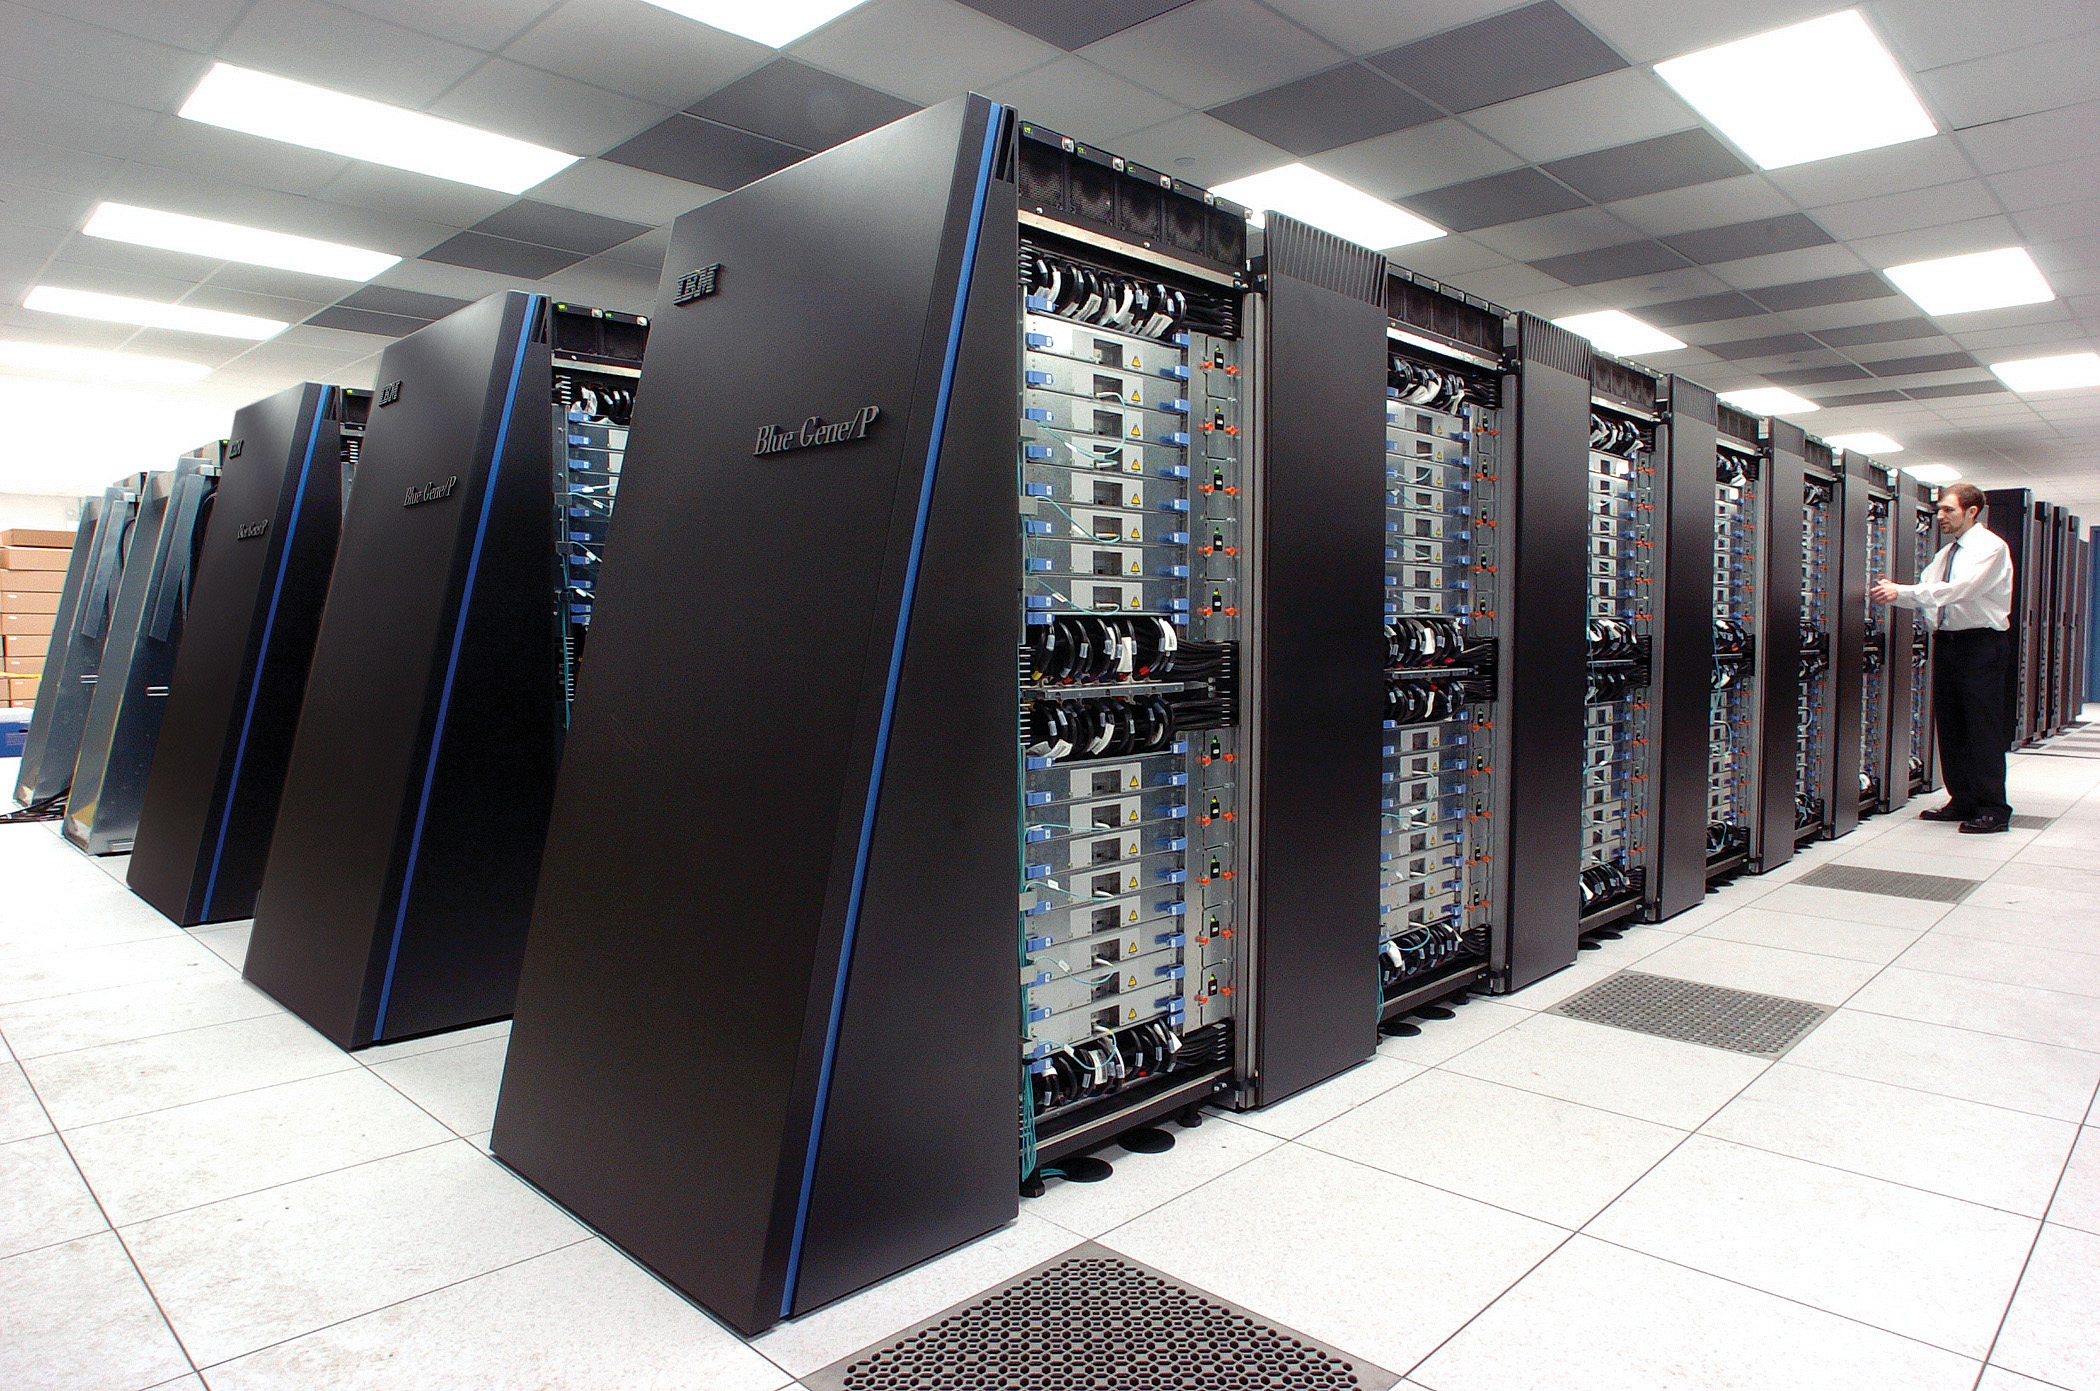
\includegraphics[width=1.00\textwidth]{pics/supercomputer.jpg}
      \end{center}
    }

    \vspace{3mm}

    Clusters usually handle long calculations with a \focus{workload manager}:\\
    \code{slurm} is one of the most popular

    \vspace{3mm}

    You will have finite disk space and CPU time:\\
    \focus{remember your limits}

    \vspace{3mm}

    Don't take too many CPUs:\\
    \focus{be mindful of others}
  \end{center}
\end{frame}

\end{document}
